\documentclass{report}
\usepackage[T1,T2A]{fontenc}
\usepackage[utf8]{inputenc}
\usepackage[russian]{babel}
\usepackage[a4paper, margin=1in]{geometry}
\usepackage{parcolumns}
\usepackage{fancyvrb}
\usepackage{hyperref}
\usepackage{unicode-math}
\usepackage{graphicx, float}
\usepackage{caption}
\usepackage{adjustbox}
\usepackage{indentfirst}

\title{
Отчет по лабораторной работе \\
{\bf "Анализ пилообразных колебаний излучения плазмы"} \\
по курсу \\
{\bf"Стохастические модели и анализ данных"}
}
\author{Мануилов Георгий, студент гр. 3640102/80201}
\date{}

\begin{document}

\maketitle

\tableofcontents

\newpage

\renewcommand\thesection{\arabic{section}}

\section{Постановка задачи}
Даны показания четырех датчиков, регистрирующих мягкое рентгеновское излучение плазмы в пяти экспериментах. В показаниях датчиков иногда наблюдаются пилообразные колебания \cite{sawtooth}, предшествующие срыву плазмы. Важно уметь вовремя детектировать такие колебания, чтобы предотвращать срыв плазмы. В связи с этим требуется:
\begin{enumerate}
    \item Представить алгоритм выделения пилообразных колебаний
    \item Оценить частоту пилообразных колебаний
\end{enumerate}

\section{Подготовка данных}
Данные представлены в бинарном формате в сжатом виде. Декодирование данных производится с помощью Python библиотеки shtRipper \cite{ripper}. Далее из декодированных данных извелкаются временные последовательности показаний датчиков, которые сохраняются в массивах NumPy \cite{numpy}.
\\

Представлены наборы данных для пяти экспериментов:
\begin{itemize}
    \item 38515
    \item 38516
    \item 38518
    \item 38521
    \item 38530
\end{itemize}

Каждый набор содержит измерения четырех датчиков:
\begin{itemize}
    \item SXR 15 мкм
    \item SXR 27 мкм
    \item SXR 50 мкм
    \item SXR 80 мкм
\end{itemize}

\section{Первичный анализ данных}
Первичный анализ данных показал, что:
\begin{itemize}
    \item Частота семплирования датчиков - 1000 кГц.
    \item Данные экспериментов 38518 и 38521 не содержат как срывов, так и участков пилообразных колебаний. Впоследствии это было подтверждено с помощью алгоритма выделения пилообразных колебаний.
    \item Следующие данные непригодны для дальнейшей обработки:
    \begin{itemize}
        \item Эксперимент 38515, датчик SXR 27 мкм
        \item Эксперимент 38516, датчик SXR 15 мкм
    \end{itemize}
\end{itemize}

\newpage

\section{Алгоритм выделения пилообразных колебаний}

\subsection{Описание алгоритма}

Предлагается следующий алгоритм для выделения пилообразных колебаний (описан алгоритм выделения для полной последовательности показаний датчика (далее сигнал), но нетрудно проверить, что алгоритм возможно применять для анализа показаний в режиме онлайн). Описание алгоритма с иллюстрациями промежуточных результатов преобразований сигнала на примере данных эксперимента 38515, датчика SXR 80 мкм:
\begin{enumerate}
    \item Выделяем область для анализа (region of interest, далее ROI). В нашем случае ROI - участок сигнала, не являющийся квазистационарным. Таким образом, ROI выделяется путем сравнения значений отсчетов с их средним значением по всему сигналу (рис. 1 и 2).
    \begin{figure}[H]
         \centering
         \captionsetup{justification=centering}
         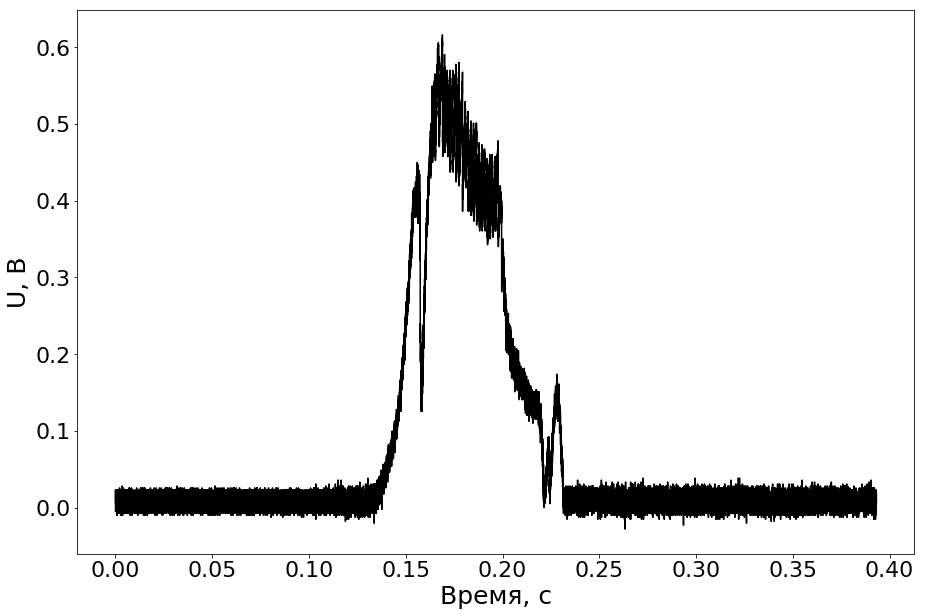
\includegraphics[width=.8\linewidth]{1_signal.png}
         \caption{Исходный сигнал}\label{Fig:Data1}
    \end{figure}
    \begin{figure}[H]
         \centering
         \captionsetup{justification=centering}
         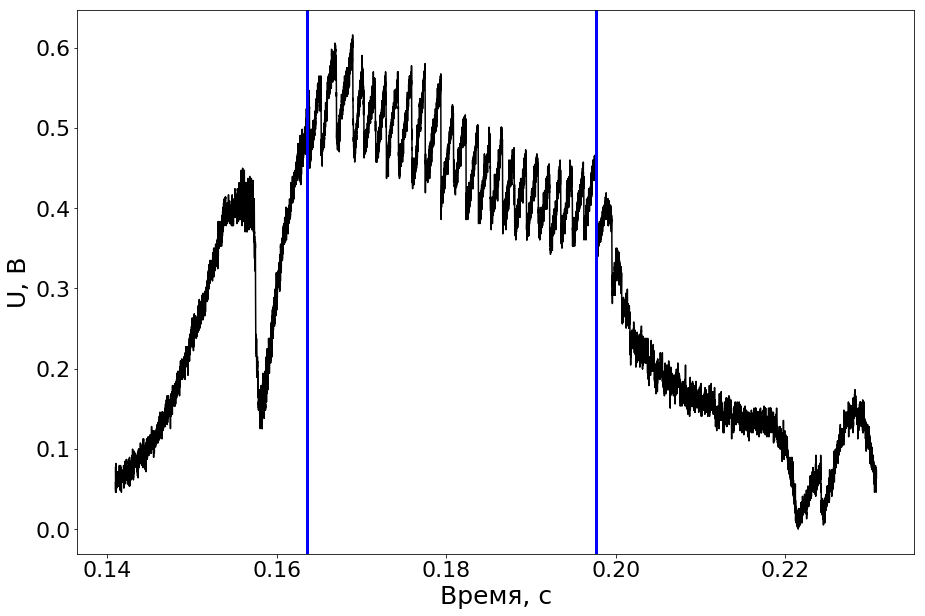
\includegraphics[width=.8\linewidth]{2_roi.png}
         \caption{ROI с выделенными началом (0.1635 с ) и концом (0.1976 с) участка пилообразных колебаний (синие прямые)}\label{Fig:Data1}
    \end{figure}
    \item Для спрямления исходного сигнала, то есть удаления низкочастотных составляющих применяем фильтр верхних частот (ФВЧ) (рис. 3).
    \begin{figure}[H]
         \centering
         \captionsetup{justification=centering}
         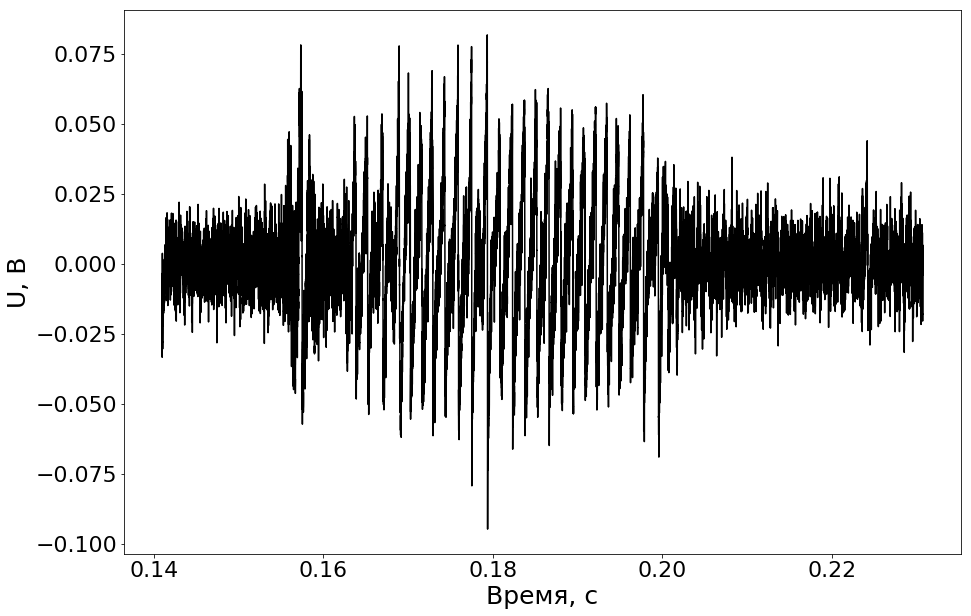
\includegraphics[width=.8\linewidth]{3_high_pass.png}
         \caption{ROI после применения ФВЧ с частотой среза 625 Гц}\label{Fig:Data1}
    \end{figure}
    \item Находим первую производную спрямленного сигнала путем применения сглаживающего цифрового дифференцирующего фильтра (ЦДФ) \cite{paper1} (рис. 4):
    \[y(n)=\sum_{k=1}^{M} \frac{1}{M(M+1)} \Delta_k, \; \Delta_k=x(n+k)-x(n-k)\]
    где $M \geq 2$ - порядок фильтра, $x(n)$ - значение $n$-ого отсчета входного сигнала, а $y(n)$ - значение $n$-ого отсчета выходного сигнала.
    \begin{figure}[H]
         \centering
         \captionsetup{justification=centering}
         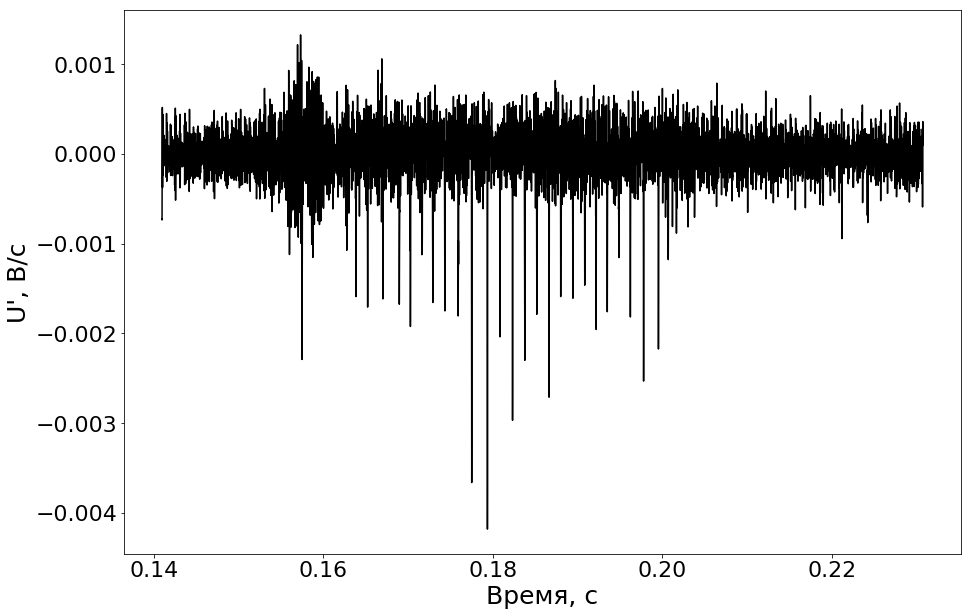
\includegraphics[width=.8\linewidth]{4_smoothed_dd1.png}
         \caption{Первая производная ROI сигнала, полученная применением ЦДФ 30 порядка}\label{Fig:Data1}
    \end{figure}
    \item Берем модуль от первой производной спрямленного сигнала (рис. 5).
    \begin{figure}[H]
         \centering
         \captionsetup{justification=centering}
         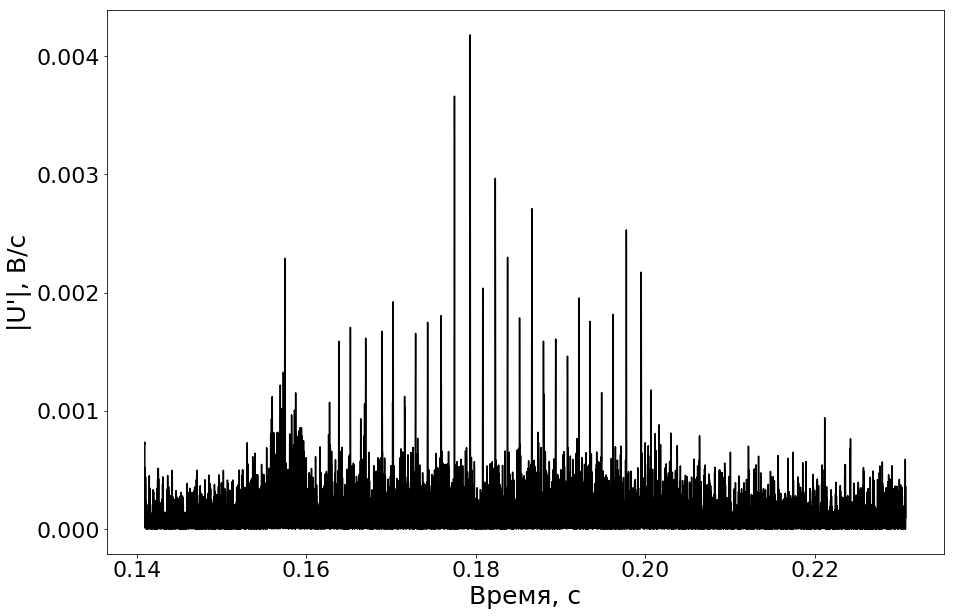
\includegraphics[width=.8\linewidth]{5_abs_du.png}
         \caption{Абсолютное значение первой производной ROI сигнала}\label{Fig:Data1}
    \end{figure}
    \item Применяем фильтр нижних частот (ФНЧ) для удаления высокочастотного шума (рис. 6).
    \begin{figure}[H]
         \centering
         \captionsetup{justification=centering}
         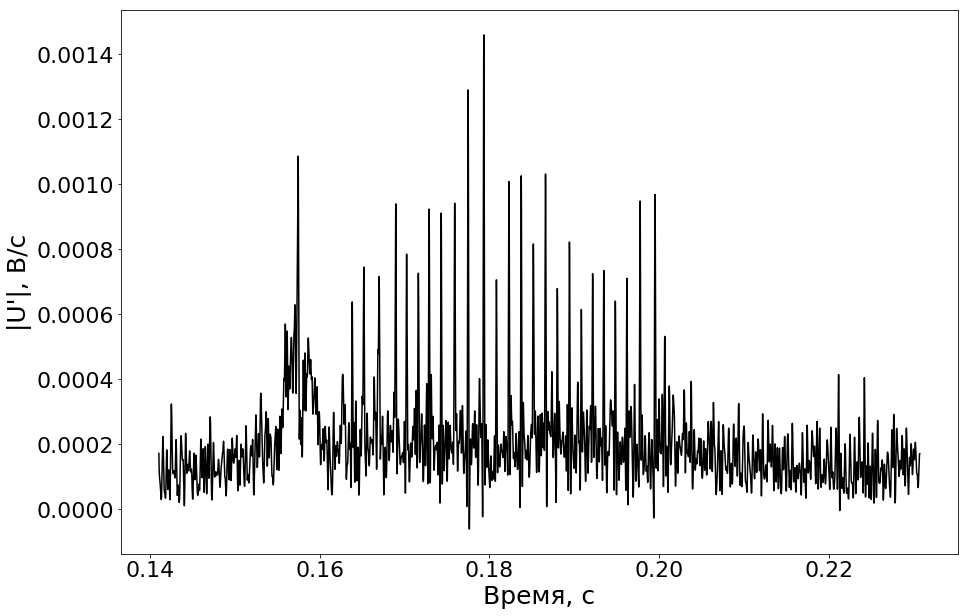
\includegraphics[width=.8\linewidth]{6_low_pass_abs_du.png}
         \caption{Абсолютное значение первой производной ROI сигнала после применения ФНЧ с частотой среза 5000 Гц}\label{Fig:Data1}
    \end{figure}
    \item Индикатором пилообразных колебаний будет служить наличие и частота появления значений сигнала выше некоторого порога (рис. 7).
    \begin{figure}[H]
         \centering
         \captionsetup{justification=centering}
         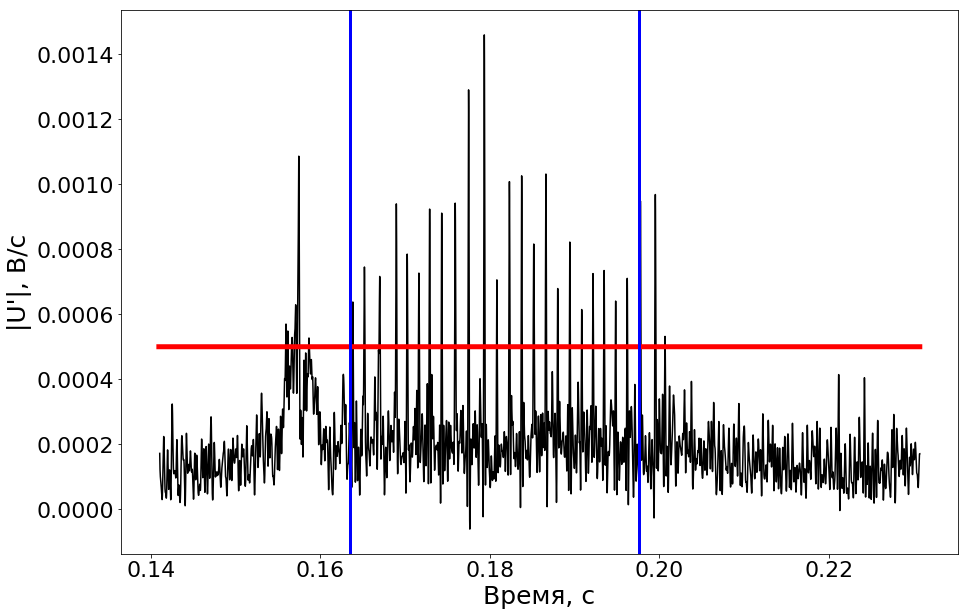
\includegraphics[width=.8\linewidth]{7_threshold.png}
         \caption{Конечный сигнал, предназначенный для обнаружения пилообразного участка по порогу 0.0005 (красная прямая), синими прямыми показаны истинные границы пилообразного участка}\label{Fig:Data1}
    \end{figure}
\end{enumerate}

Как видно по рис. 7 предложенный алгоритм позволяет достаточно точно определять участок с пилообразными колебаниями в сигнале датчика: большая часть значений выше порога действительно принадлежит искомому участку. Достаточно добавить подсчет числа пиков в некотором скользящем окне, и выброс, расположенный около 0.159 с также будет отфильтрован.
\\

Также стоит отметить, что алгоритм без проблем можно применять (после некоторой переработки шагов, в которых применяются фильтры) в реальном времени, так как он не требует для работы всей последовательности наблюдений.
\\

В целом алгоритм хорошо показал себя на всех имеющихся данных, кроме экспериментов 38518 и 38521, в которых пилообразные колебания не были зафиксированы как алгоритмом, так и визуально. Подобный алгоритм также описан в работе \cite{paper2}, и судя по всему, успешно применяется на практике.
\\

Стоит отметить, что на идеальных данных (например, эксперимент 38515, датчик SXR 80 мкм) алгоритм можно применять, пропуская шаги 3-5: спрямление сигнала позволяет точно зафиксировать участок пилообразных колебаний по порогу. Последовательность обработки данных для указанного эксперимента показана на рис. 8 и 9.

\begin{figure}[H]
     \centering
     \captionsetup{justification=centering}
     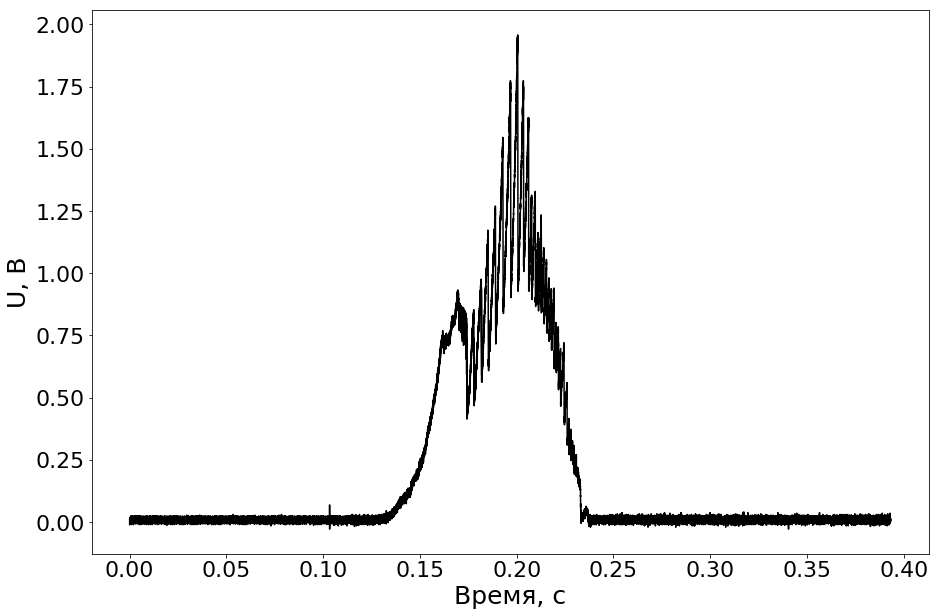
\includegraphics[width=.8\linewidth]{9_signal_38516.png}
     \caption{Исходный сигнал для эксперимента 38515, датчика SXR 80 мкм}\label{Fig:Data1}
\end{figure}
\begin{figure}[H]
     \centering
     \captionsetup{justification=centering}
     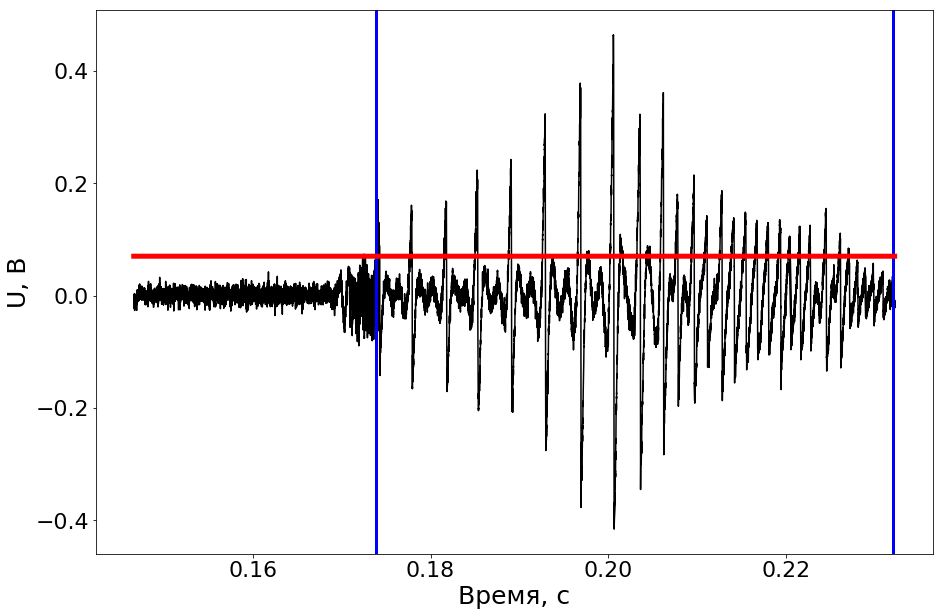
\includegraphics[width=.8\linewidth]{9_signal_38516_high_pass.png}
     \caption{Выделение пилообразного участка для эксперимента 38515, датчика SXR 80 мкм}\label{Fig:Data1}
\end{figure}

\newpage

\subsection{Параметры алгоритма}

Алгоритм параметризуется следующими величинами:
\begin{itemize}
    \item Порядком ЦДФ
    \item Пороговым значением
\end{itemize}

Стоит отметить, что параметры ФВЧ на шаге №2 и ФНЧ на шаге №3 также могут зависеть от условий эксперимента, однако такой зависимости не наблюдалось при обработке предоставленных данных.
\\

Можно предложить альтернативу последнему шагу, которая не требует задания порогового значения, повышая таким образом устойчивость алгоритма. Такая альтернатива - оценка плотности распределения локальных максимумов в некотором окне: во время пилообразных колебаний плотность понижается (рис. 10).
\begin{figure}[H]
     \centering
     \captionsetup{justification=centering}
     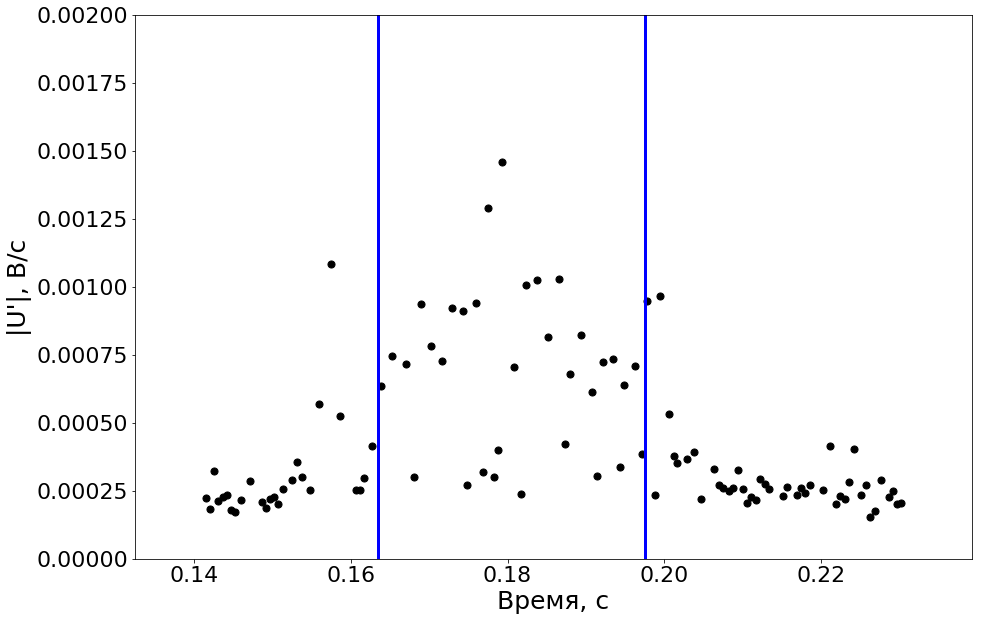
\includegraphics[width=.8\linewidth]{8_peaks.png}
     \caption{Локальные максимумы конечного сигнала в окне с размером 400 отсчетов (0.0004 с)}\label{Fig:Data1}
\end{figure}

\newpage

\section{Оценка частоты пилообразных колебаний}
После выделения участка пилообразных колебаний можно попробовать оценить их частоту, а точнее ее эволюцию. Для решения подобных задач широко применяются два способа: преобразование Фурье и анализ автокорреляционной функции.
\\

Применение первого способа к имеющимся данным затруднительно, так как интересующие нас частоты лежат в полосе от 0 до 1 кГц, в то время как переход из временной области в частотную с помощью преобразования Фурье дает нам спектр от 0 до 500 кГц. Кроме того, сигнал сильно зашумлен, поэтому даже после применения ФНЧ и ФВЧ выделить собственные частоты пилообразных колебаний не представляется возможным без априорных знаний об искомой полосе частот.
\\

Второй способ мог бы решить задачу, однако его экстраполяция на случай с переменной частотой, вообще говоря, нетривиальна.
\\

Для решения задачи с учетом специфики предоставленных данных предлагается следующий простой алгоритм (на рис. 11-13 показаны иллюстрации шагов алгоритма для данных эксперимента 38515, датчика SXR 80 мкм):
\begin{enumerate}
    \item Спрямляем участок, содержащий пилообразные колебания с помощью ФВЧ с частотой среза 250 Гц.
    \item Удаляем высокочастотные шумы спрямленного сигнала с помощью ФНЧ с частотой среза 200 Гц.
    \item Ищем все точки пересечения сигнала с осью абсцисс.
    \item Вычитаем полученные значения друг из друга через одного, получая мгновенные периоды колебаний.
    \item Из периодов получаем мгновенные частоты, то есть функцию частоты от времени.
    \item Для сглаживания полученной функции применяем любой сглаживающий фильтр, например, скользящее среднее с окном 5.
\end{enumerate}

\begin{figure}[H]
     \centering
     \captionsetup{justification=centering}
     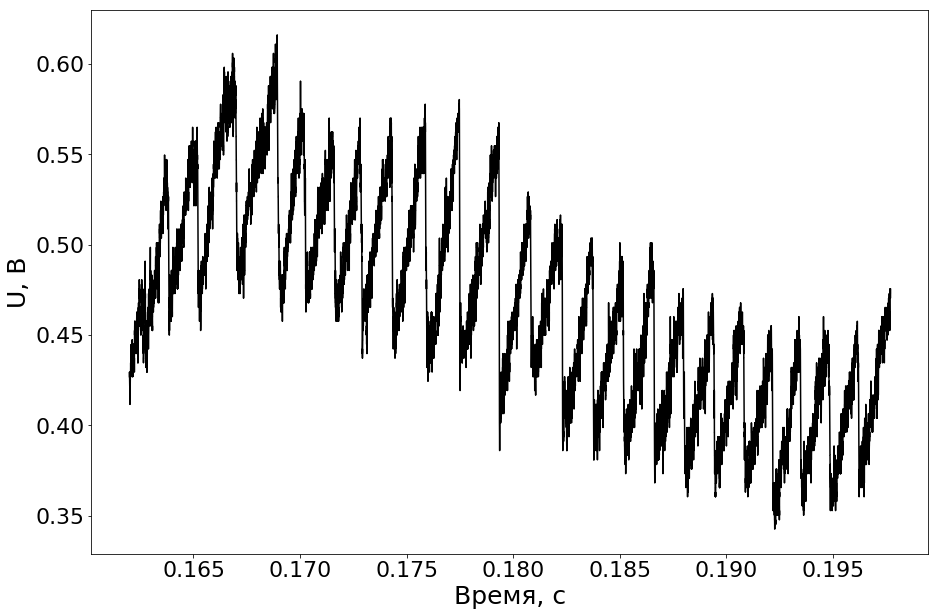
\includegraphics[width=.8\linewidth]{f1_roi.png}
     \caption{Выделенный участок пилообразных колебаний в данных эксперимента 38515, датчика SXR 80 мкм}\label{Fig:Data1}
\end{figure}
\begin{figure}[H]
     \centering
     \captionsetup{justification=centering}
     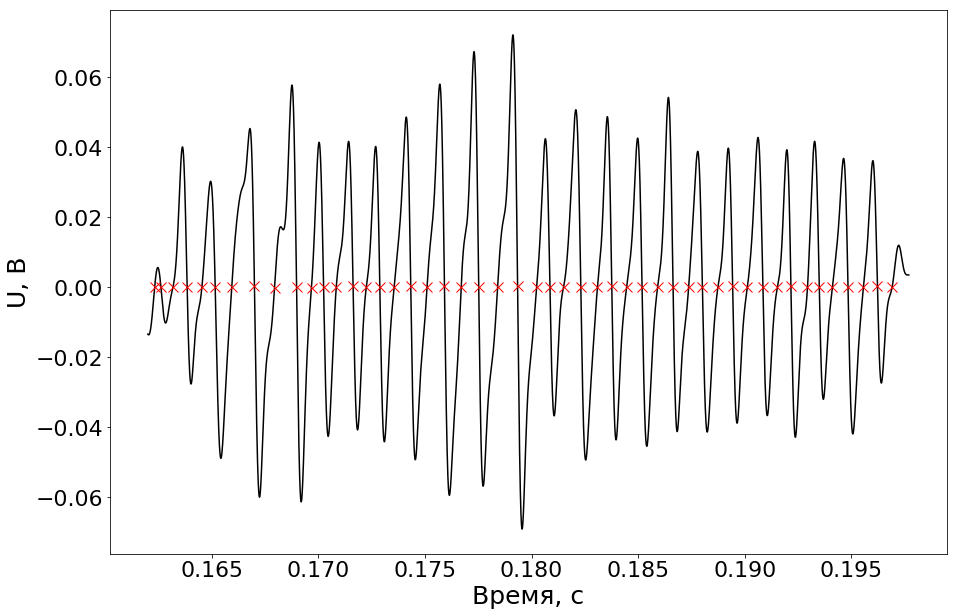
\includegraphics[width=.8\linewidth]{f2_filter_zero_crossings.png}
     \caption{Спрямленный и отфильтрованный участок сигнала пилообразных колебаний для эксперимента 38515, датчика SXR 80 мкм, красным отмечены точки пересечения с осью абсцисс}\label{Fig:Data1}
\end{figure}
\begin{figure}[H]
     \centering
     \captionsetup{justification=centering}
     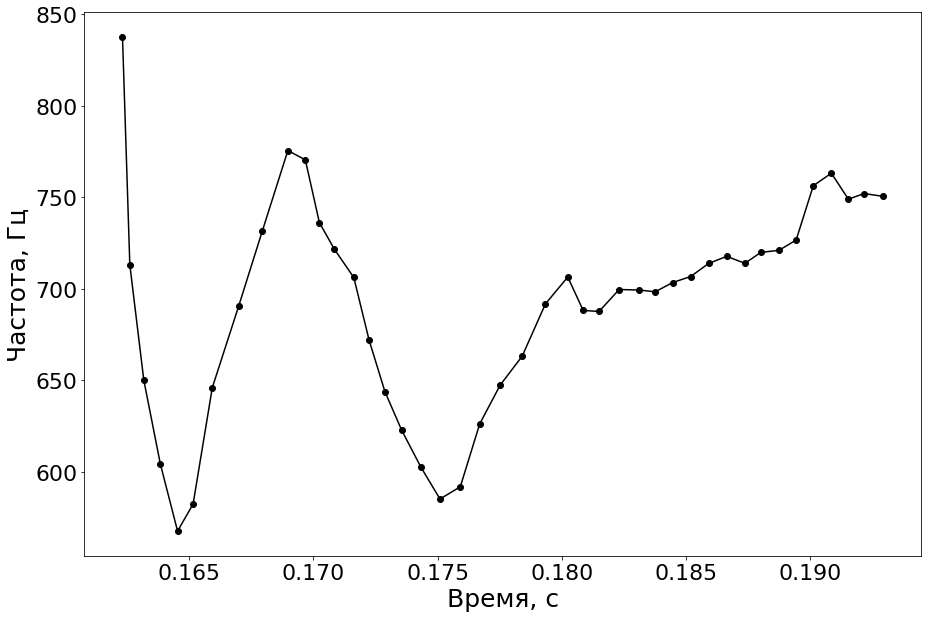
\includegraphics[width=.8\linewidth]{f3_freq.png}
     \caption{Полученная функция частоты от времени для участка пилообразных колебаний для эксперимента 38515, датчика SXR 80 мкм}\label{Fig:Data1}
\end{figure}

\newpage

На рис. 14-16 показаны графики функций частоты от времени для участков пилообразных колебаний для всех датчиков в экспериментах 38515, 38516 и 38530.

\begin{figure}[H]
     \centering
     \captionsetup{justification=centering}
     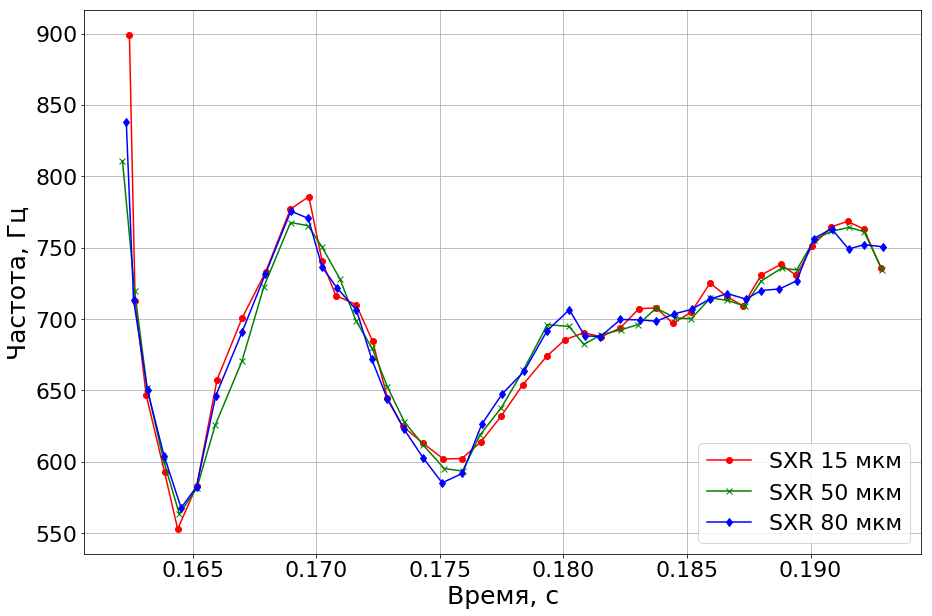
\includegraphics[width=.8\linewidth]{38515_freq.png}
     \caption{График функци частоты от времени для участков пилообразных колебаний для всех датчиков в эксперименте 38515}\label{Fig:Data1}
\end{figure}
\begin{figure}[H]
     \centering
     \captionsetup{justification=centering}
     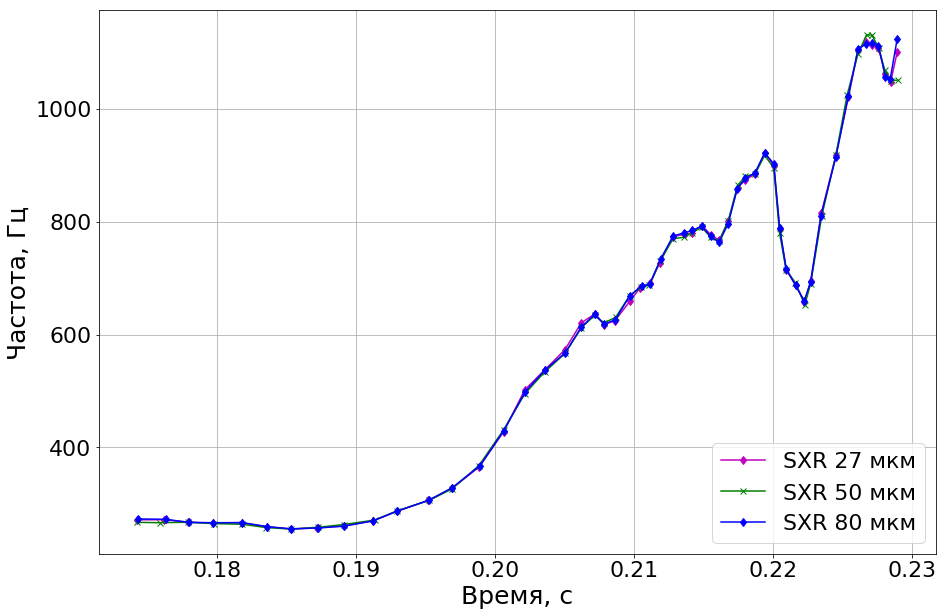
\includegraphics[width=.8\linewidth]{38516_freq.png}
     \caption{График функци частоты от времени для участков пилообразных колебаний для всех датчиков в эксперименте 38516}\label{Fig:Data1}
\end{figure}
\begin{figure}[H]
     \centering
     \captionsetup{justification=centering}
     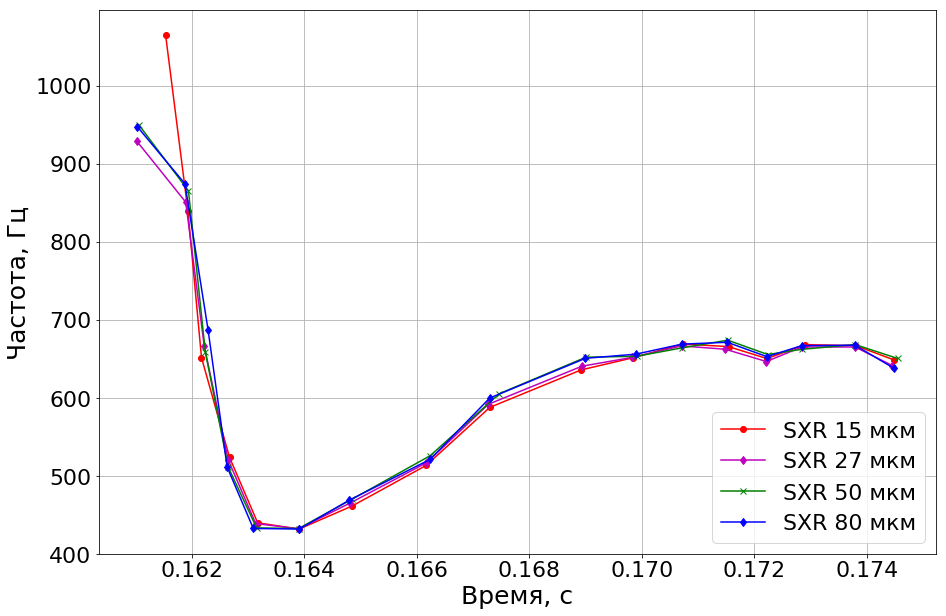
\includegraphics[width=.8\linewidth]{38530_freq.png}
     \caption{График функци частоты от времени для участков пилообразных колебаний для всех датчиков в эксперименте 38530}\label{Fig:Data1}
\end{figure}

\newpage

\section{Выводы}
Представлены алгоритмы, решающие поставленные задачи. Исходный код примеров реализаций алгоритмов, позволяющий воспроизвести результаты, приведенные в данном отчете, доступен в репозитории [6].
\\

Алгоритм для детектирования пилообразных колебаний продемонстрировал удовлетворительную точность. Кроме того, в литературе были обнаружены упоминания алгоритмов, основанных на похожих принципах, а также свидетельства их успешного применения на практике, что говорит о правильно выбранном направлении разработки.
\\

Алгоритм для выделения частот пилообразных колебаний также дает удовлетворительный результат по крайней мере на предоставленных данных. Стоит отметить, что характер пилообразных колебаний хоть и одинаков для каждого из датчиков в одном эксперименте, но тем не менее очень отличается от эксперимента к эксперименту. Отличия можно заметить в длительности участка (от 0.019 до 0.058 с), во внешнем виде и характере функции зависимости частоты от времени, а также в интервале частот (от 400 до 1100 Гц). Тем не менее, если пренебречь изменением частоты на участке пилообразных колебаний, то можно сказать, что средняя частота пилообразных колебаний для всех экспериментов лежит в интервале от 600 до 700 Гц.

\begin{thebibliography}{9}

\bibitem{sawtooth} 
Tokamak sawtooth
\\\texttt{https://en.wikipedia.org/wiki/Tokamak\_sawtooth}

\bibitem{ripper} 
Библиотека shtRipper
\\\texttt{https://gitlab.spectraltech.ru/Rezenter/shtRipper}

\bibitem{numpy} 
Библиотека NumPy
\\\texttt{https://numpy.org}

\bibitem{paper1} 
S. Usui, I. Amidror.
\textit{Digital Low-Pass Differentiation for Biological Signal Processing}. 
IEEE Transactions on Biomedical Engineering, vol. BME-29, issue 10, 1982, pp. 686-693

\bibitem{paper2} 
Felici, F. and Le, H.B. and Paley, J.I. and Duval, B. and Coda, S. and Moret, J.-M and Bortolon, Alessandro and Federspiel, Lucia and Goodman, T. and Hommen, Gillis and Karpushov, Alexander and Piras, F. and Pitzschke, Andreas and Romero, Jesús and Sevillano, M. and Sauter, O. and Vijvers, Wouter.
\textit{Development of real-time plasma analysis and control algorithms for the TCV tokamak using SIMULINK}.
Fusion Engineering and Design, vol. 89, issue 3, 2014, pp. 165-176

\bibitem{code} 
Примеры реализаций описанных алгоритмов
\\\texttt{https://github.com/dev0x13/plasma\_sawooth\_analysis}
\end{thebibliography}

\end{document}
